\documentclass[conference]{IEEEtran}
\usepackage{caption}
\usepackage{graphicx}
\usepackage{epstopdf}
\usepackage{subcaption}
\usepackage{cite}
\usepackage{amsmath}
\usepackage{fancyhdr}
% correct bad hyphenation here
\hyphenation{op-tical net-works semi-conduc-tor}


\begin{document}

\title{Bangla Handwritten Numeral Character Recognition Using Directional Pattern}


\author{
	\IEEEauthorblockN{Talha Ibn Aziz\IEEEauthorrefmark{1},
		Al Shahriar Rubel\IEEEauthorrefmark{2},
		Md Sirajus Salekin\IEEEauthorrefmark{3} and
		Rafsanjany Kushol\IEEEauthorrefmark{4}
	}
	\IEEEauthorblockA{
		\IEEEauthorrefmark{1}\IEEEauthorrefmark{2}\IEEEauthorrefmark{4}
		Department of Computer Science and Engineering, Islamic University of Technology, Dhaka, Bangladesh\\
		\IEEEauthorrefmark{3}
		Department of Computer Science and Engineering, University of South Florida, Florida, United States
		}
	\IEEEauthorblockA{
		\IEEEauthorrefmark{1}talhaibnaziz@iut-dhaka.edu,
		\IEEEauthorrefmark{2}alshahriar@iut-dhaka.edu,
		\IEEEauthorrefmark{3}salekin@mail.usf.edu and
		\IEEEauthorrefmark{4}kushol@iut-dhaka.edu
	}
}


% make the title area
\maketitle

\thispagestyle{fancy}
\pagenumbering{gobble} %%removing page number
\renewcommand{\headrulewidth}{0pt}

\fancyhead[R]{2017 20th International Conference of Computer and Information Technology (ICCIT), 22-24 December, 2017}
\fancyfoot[L]{978-1-5386-1150-0/17/\$31.00~\copyright 2017 IEEE}
%\fancyfoot[R]{ISBN 978-1-5386-1150-0}


\begin{abstract}
Handwritten character recognition has become a challenging and interesting field in the recent days due to its complex character shapes and huge pragmatic applications. A lot of research is already done and underway on English alphabets and numerals recognition. But in case of Bangla, even being the fifth largest spoken language in the world, has not undergone that much research. Besides, different complex shape of Bangla character makes the recognition more challenging. In this paper, we propose a directional pattern approach for feature extraction of Bangla numeric characters which attains a high accuracy of recognition. We use Local Directional Pattern (LDP) and Gradient Directional Pattern (GDP) for feature extraction and then two well-known machine learning algorithms, K-Nearest Neighbour (KNN) and Support Vector Machine (SVM), to classify the numeric character. We also ensemble the pattern oriented results to enhance the accuracy. Experimental results on the benchmark dataset CMATERdb 3.1.1 demonstrates an astounding recognition rate of accuracy 95.62\% without preprocessing the data.
\end{abstract}

\begin{IEEEkeywords}
Bangla Character Recognition, Bangla Digit Recognition, Directional Pattern, Local Directional Pattern, Gradient Directional Pattern
\end{IEEEkeywords}

\IEEEpeerreviewmaketitle


\section{Introduction}
Handwritten character recognition is a process where a machine tries to interpret images of characters written by hand. It represents a numeral or an alphabet. It has many applications including reading documents, hand-held notebooks, touch screens, optical scanning by intelligent systems etc. Hence researchers are still trying to improve the handwritten character recognition algorithms. However, Bangla handwritten character recognition has not been extensively studied as English handwritten character recognition. There are some attempts of classification which are impressive. Moreover, most of the papers earlier lacked databases. So self-written characters or self-taken images were used which lacked the authenticity and variation that a standard database possessed. But that deficit is now not present anymore because there are some benchmark databases such as ISI \cite{2006isi} and CMATERdb\cite{2009cmater}.


Research works on Bangla handwritten character recognition can be broadly divided into two categories. One is Bangla handwritten character recognition and another one is Bangla handwritten numerals or digit recognition. Although There were some noteworthy works on Bangla handwritten character recognition \cite{1998BHCR, 2004BHCR}, Bangla handwritten numerals recognition did not improve much. Later on, since benchmark data set such as ISI \cite{2006isi} and CMATERdb \cite{2009cmater} developed, a lot of researchers are motivated to work on the Bangla handwritten numerals recognition. U. Pal et al. \cite{2007gradientfeature} used gradient feature to recognize Bengali compound characters. They didn't use any standard data set but gained an accuracy of 85.90\% which is quite high for compound characters using 5-fold cross validation. M. Z. Hossain et al.\cite{2011rapidfeature} used a rapid feature extraction called Celled Projection (CP) method along with different classifiers and gained an accuracy of 94.12\%. They collected data from 120 writers forming a data set of 12000 images. N. Das et al. \cite{2012geneticalgorithm} used a Genetic algorithm on seven sets of local region. O. Surinta \cite{2013contourangular} proposed a contour angular technique to find out the patterns. Majority voting method is used to identify the best recognition. H. A. Khan et al. \cite{2014sparseclassifier} used Sparse Representation of classifier where they assumed that test data is the linear combination of the training data using its native class. Recently, Pattern oriented feature extraction such as LBP \cite{2002LBP}, LDP \cite{2010LDP}, GDP \cite{2012GDP}, POMF \cite{2017POMF} have become popular due to its robustness across the neighbourhood regions. Already some of the researchers \cite{2015LBP} achieved better recognition rate using pattern oriented features on Bangla handwritten digit recognition.

In this paper, we propose an ensemble method using LDP and GDP to provide a pattern oriented robust approach for Bangla handwritten numeral recognition. Two well-known classifiers, K-Nearest Neighbour (KNN) \cite{1967KNN} and Support Vector Machine (SVM) \cite{1995SVM}, are used for the ensemble method to classify properly using the majority voting. 

\section{Directional Pattern}
Directional Pattern is a feature extracting approach \cite{2002LBP,2010LDP,2012GDP,2017POMF} to capture the changes of pixels surrounding a specific pixel of an image. Thus the changed value does not depend only on its own data but also its adjacent pixels. It rearranges the values of the raw data and assigns weighted values to each previous location using variances in the data surrounding it. In this paper, we have used two promising directional pattern approach, Local Directional Pattern (LDP) \cite{2010LDP} and Gradient Directional Pattern (GDP) \cite{2012GDP} for recognizing Bangla numeral character efficiently.

\subsection{Local Directional Pattern (LDP)}
Local Directional Pattern (LDP) \cite{2010LDP} is motivated by the edge response. It enhances the Local Binary Pattern (LBP) \cite{2002LBP} incorporating the directional edge response by Kirsch Masks. It is a robust micro-pattern compared to LBP \cite{2002LBP} since it considers the surrounding edge responses. As a result, it easily suppresses the noise.There are eight directional masks which are applied to the image pixel by pixel from left to right on overlapping blocks. For a particular central pixel of a block, eight directional edge responses $m_i$ where $i = \{0, 1, 2,...,7\}$ are calculated for different Krish masks $M_i$. Different directional Krish masks are shown in the following matrices as East ($M_0$), North-East ($M_1$), North ($M_2$), North-West ($M_3$), West ($M_4$), South-West ($M_5$), South ($M_6$) and South-East ($M_7$) respectively.

\begin{center}
	\[
	M_0 = 
	\begin{bmatrix}
	-3 & -3 & +5 \\
	-3 & 0 & +5 \\
	-3 & -3 & +5
	\end{bmatrix}
	%East
	M_1 = 
	\begin{bmatrix}
	-3 & +5 & +5 \\
	-3 & 0 & +5 \\
	-3 & -3 & -3
	\end{bmatrix}
	%North East
	\]
	\[
	M_2 = 
	\begin{bmatrix}
	+5 & +5 & +5 \\
	-3 & 0 & -3 \\
	-3 & -3 & -3
	\end{bmatrix}
	%North
	M_3 = 
	\begin{bmatrix}
	+5 & +5 & -3 \\
	+5 & 0 & -3 \\
	-3 & -3 & -3
	\end{bmatrix}
	%North West
	\]
	\[
	M_4 = 
	\begin{bmatrix}
	+5 & -3 & -3 \\
	+5 & 0 & -3 \\
	+5 & -3 & -3
	\end{bmatrix}
	%West
	M_5 = 
	\begin{bmatrix}
	-3 & -3 & -3 \\
	+5 & 0 & -3 \\
	+5 & +5 & -3
	\end{bmatrix}
	%South West
	\]
	\[
	M_6 = 
	\begin{bmatrix}
	-3 & -3 & -3 \\
	-3 & 0 & -3 \\
	+5 & +5 & +5
	\end{bmatrix}
	%South
	M_7 = 
	\begin{bmatrix}
	-3 & -3 & -3 \\
	-3 & 0 & +5 \\
	-3 & +5 & +5
	\end{bmatrix}
	%South East
	\]
	
\end{center}

The values gained from applying the mask gives us a matrix of 8 values which are placed in the 8 directions except for the center. This matrix is then used to generate a binary pattern. The attained values are sorted and the first $k$ values are assigned $1$ and the rest are assigned $0$. The value of $k$ can be selected as per need of performance. LDP code is generated as the following

\begin{equation}
LDP_{k}=\sum_{i=0}^{i=7} b_i(m_i - m_k)2^i
\end{equation}
where,
\begin{equation}
b_i(x)=
\begin{cases}
1 & x \ge 0\\
0 & x < 0
\end{cases}
\end{equation}

Here, $m_k$ is the $k$-th most significant directional response. Using this binary pattern, the number that is formed is placed at the center. One example are shown below where - $M_0$ is considered for the least significant bit (LSB) and $M_7$ for the most significant bit (MSB) for binary pattern.

Step 1. All the 8 directional Krish masks are applied and a new matrix is formed\\

\begin{center}
	\begin{tabular}{|c|c|c|}
		\hline
		35 & 123 & 79 \\
		\hline
		16 & 10 & 201 \\
		\hline
		101 & 56 & 99 \\
		\hline
	\end{tabular}
	$\Longrightarrow$masks$\Longrightarrow$
	\begin{tabular}{|c|c|c|}
		\hline
		-738 & -234 & 1094 \\
		\hline
		-914 & X & 902 \\
		\hline
		-746 & -82 & 718 \\
		\hline
	\end{tabular}
\end{center}

Step 2. The attained values form the center value\\

\begin{center}
	\begin{tabular}{|c|c|c|}
		\hline
		$M_3$ & $M_2$ & $M_1$ \\
		\hline
		$M_4$ & X & $M_0$ \\
		\hline
		$M_5$ & $M_6$ & $M_7$ \\
		\hline
	\end{tabular}
	$\Longrightarrow$
	\begin{tabular}{|c|c|c|}
		\hline
		0 & 0 & 1 \\
		\hline
		0 & X & 1 \\
		\hline
		0 & 0 & 1 \\
		\hline
	\end{tabular}
\end{center}


Step 3. LDP value = $2^0$+$2^1$+0+0+0+0+0+$2^7$ = 131. Thus, the center value is replaced by the new value

\begin{center}
	\begin{tabular}{|c|c|c|}
		\hline
		35 & 123 & 79 \\
		\hline
		16 & 131 & 201 \\
		\hline
		101 & 56 & 99 \\
		\hline
	\end{tabular}
\end{center}

\subsection{Gradient Directional Pattern (GDP)}
Gradient Directional Pattern (GDP) \cite{2012GDP} is another directional pattern which uses gradient values for micro-pattern. Although LDP \cite{2010LDP} suppresses the noise reduction it generates inconsistent codes in uniform and near-uniform regions. But GDP tries to solve this problem introducing the gradient direction angles. This is almost same as LDP except that it works with the gradients of the pixels rather than the grayscale values. It uses Sobel Masks to find out the horizontal $G_x$ and vertical $G_y$ gradient direction. Sobel Masks are shown below.

\begin{center}
	\[
	X - Direction\quad Kernel, G_x = 
	\begin{bmatrix}
	+1 & 0 & -1 \\
	+2 & 0 & -2 \\
	+1 & 0 & -1
	\end{bmatrix}
	\]
	\[
	Y - Direction\quad Kernel, G_y = 
	\begin{bmatrix}
	+1 & +2 & +1 \\
	0 & 0 & 0 \\
	-1 & -2 & -1
	\end{bmatrix}
	\]
\end{center}


Later on, gradient angle is computed from the $G_x$ and $G_y$ as follows.

\begin{equation}
 GA (x,y) = tan^{-1}(G_y/G_x)
\end{equation}

Here, $GA (x,y)$ represents the gradient direction angle of the pixel (x,y). The values gained from gradient angles gives us a matrix of 9 values. Then this matrix is used to generate a binary pattern. The difference of the center gradient angle values with its adjacent pixel values are compared and placed a $0$ if it is greater to a threshold $t$ and $1$ if not. This threshold $t$ is to be found out experimentally. The value usually varies from $20^0$ to $50^0$. GDP code is generated as the following

\begin{equation}
GDP ({x_c, y_c})=\sum_{p=0}^{p-1} w (GA_p - GA_c) 2^p
\end{equation}
where,
\begin{equation}
 w (GA_p - GA_c) =
\begin{cases}
1 & GA_c - t \leq GA_p \leq GA_c + t\\
0 & otherwise
\end{cases}
\end{equation}

Here, $GA_c$ is the gradient direction angle of the centre pixel ($x_c$, $y_c$), $GA_p$ is the angles of its neighbors, and $t$ is a user-specified threshold.

An example is shown for GDP calculation using the a $3 \times 3$ matrix as follows.

Step 1. - The image is convolved using the kernels. The center value is attained.

\begin{center}
	\[
	\begin{split}
	G_x & = \Bigg(
	\begin{bmatrix}
		+1 & 0 & -1 \\
		+2 & 0 & -2 \\
		+1 & 0 & -1
	\end{bmatrix}
	*
	\begin{bmatrix}
		35 & 123 & 79 \\
		16 & 10 & 201 \\
		101 & 56 & 99
	\end{bmatrix}\Bigg) \\
	& = -35 + 0 + 79 - 32 + 0 + 402 - 101 + 0 + 99 \\
	& = 412
	\end{split}
	\]
	
	\[
	\begin{split}
	G_y & = \Bigg(
	\begin{bmatrix}
	+1 & +2 & +1 \\
	0 & 0 & 0 \\
	-1 & -2 & -1
	\end{bmatrix}
	*
	\begin{bmatrix}
	35 & 123 & 79 \\
	16 & 10 & 201 \\
	101 & 56 & 99
	\end{bmatrix}\Bigg) \\
	& = -35 - 246 - 79 + 0 + 0 + 0 + 101 + 56 + 99 \\
	& = -104
	\end{split}
	\]
\end{center}

Step 2. - Calculating Approximate Gradient Value\\
\[
	GA (2,2) = tan^{-1}(-104/412) = -14.167
\]

Step 3. - Perform the steps 2 and 3 of LDP. We did the previous steps on a $3 \times 3$ matrix so we got 1 center value. When performed on the whole image of $m \times n$ size, a matrix of $(m-1) \times (n-1)$ is attained on which then this step is performed taking each $3 \times 3$ block at a time.


\section{Proposed Method}
In this paper, an ensemble method containing the directional pattern is proposed. Feature extraction process is performed through the micro-pattern of LDP and GDP. Then KNN and SVM classifiers are used to generate the ensemble approach. Finally, the maximum voted class is considered for the predicted class of the test sample. The overall process can be explained in two steps: features extraction through directional pattern and ensemble approach for classification and recognition.

\subsection{Feature Extraction using Directional Pattern}
In our experiments, any noise reduction or any other sort of pre-processing on the images is not performed. Rather we directly used the directional pattern feature extraction methods on the images. Even without any noise cancellation or slant correction or size normalization, the proposed method performs excellently achieving a high accuracy. We used the whole $32\times32$ bitmap image as the raw data and input for our methods. Two feature extraction methods - LDP and GDP are performed. The image is divided into the overlapping blocks and LDP and GDP is applied. Finally, the whole image was divided into some non-overlapping zones. From each of the zones, histograms are generated and concatenated one after another to produce the feature vector. 

\subsection{Ensemble Approach for classification}
Two robust classifiers KNN \cite{1967KNN} and SVM \cite{1995SVM} are used for ensemble methods. Experimentally, we have found that KNN and SVM classifier works better on the image with LDP and GDP. The KNN considers each value of the vector as a coordinate and performs Euclidean distance calculation to classify each test sample with respect to each training sample. The value of $k = 3$ for KNN gave the best classification in our case. On the other hand, multi-class SVM with a quadratic kernel is found to give the best performance in our experiment. Three combinational approaches are proposed. If more than one of the three approaches gave the same results then we took that as the final result.

\section{Experimental Analysis and Discussion}

\subsection{Dataset and Experimental Setup}
In our experiments, the CMATERdb 3.1.1 \cite{2009cmater} database which contains 6000 images of Bengali numerals were used. For each digit, there are 600 images each being bitmap images of size $32 \times 32$. These images are converted into grayscale images before feature extraction. Some sample images are shown in Fig \ref{fig:bangladigits}.

\begin{figure}
	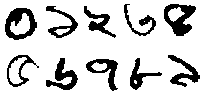
\includegraphics[width=\linewidth]{digits.png}
	\caption{Bitmap images of the benagli digits from CMATERdb 3.1.1}
	\label{fig:bangladigits}
\end{figure}

6-fold cross validation was performed on the 6000 data sets where each fold contains 1000 images. We focused more on avoiding over-fitting than on accuracy so that the classifier would be more universal, but this decreased the accuracy with respect to some separate data sets created arbitrarily. The highest accuracy for the separate folds was found to be 96\% when GDP with $t = 28.5$ for $6\times6$ zones was applied.

\subsection{Result Analysis and Comparison}
In our experiment, KNN is performed on different zone configurations of GDP and LDP. KNN yields better results on the image when the value of $k$ is odd and the best results are obtained from $k = 3$. As we have shown in Table \ref{table_LDP_KNN}, the best accuracy is found by LDP which is performed on region division of $4 \times 4$ which is 93.42\%. However, for $k = 1$ and $k = 5$ it produces good rates of recognition compared to $k = 2$ and $k = 4$. The $2\times2$ zone produces an image with 4 regions, each giving a histogram of size 256. Thus the whole image produces a feature vector of dimensions $4\times256$. Similarly, the next two region divisions give feature vectors of sizes respectively $16\times256$ and $64\times254$. When SVM is performed on the same image after LDP is done, the accuracies are 92.85\% and 92.4333\% respectively for zones $4\times4$ and $8\times8$. 

\begin{center}
	\captionof{table}{Zone-wise accuracy of LDP for KNN}
	\label{table_LDP_KNN}
	\begin{tabular}{cccc}
		\hline
		Classifier & LDP($2\times2$) & LDP($4\times4$) & LDP($8\times8$) \\
		\hline
		KNN (k=5) & 88.3333 & 93.2167 & 92.9833\\
		KNN (k=4) & 87.5500 & 92.7333 & 92.7333\\
		KNN (k=3) & 88.7500 & 93.4167 & 93.2833\\
		KNN (k=2) & 85.2167 & 91.2500 & 91.6667\\
		KNN (k=1) & 88.3333 & 93.2167 & 92.9833\\
		\hline
	\end{tabular}
\end{center}

In Table \ref{table_GDP_KNN}, we have shown the results of KNN with different values of $k$, after GDP is applied with $t = 28.5$ for different zones. The odd values of $k$ give better results than even values because an odd number of results have a better probability of forming a majority while even values can result in ties and thus decrease classification accuracy. However, the zones of $6\times6$ give better recognition rate than all the corresponding zones except for $k = 4$ in which case $5\times5$ is more accurate than $6\times6$.

\begin{center}
	\captionof{table}{Zone-wise accuracy of GDP (t = 28.5) for KNN}
	\label{table_GDP_KNN}
	\begin{tabular}{cccc}
		\hline
		Classifier & GDP($5\times5$) & GDP($6\times6$) & GDP($10\times10$)\\
		\hline
		KNN (k=5) & 93.17 & 93.90 & 93.88\\
		KNN (k=4) & 91.53 & 93.32 & 93.17\\
		KNN (k=3) & 93.43 & 94.05 & 93.88\\
		KNN (k=2) & 92.52 & 92.22 & 91.98\\
		KNN (k=1) & 93.18 & 93.75 & 93.52\\
		\hline
	\end{tabular}
\end{center}

The performance of GDP and LDP for different zones is also shown in Table \ref{table_LDP_GDP}. GDP provides better classification accuracy than LDP.

\begin{center}
	\captionof{table}{Overall zone-wise Accuracy}
	\label{table_LDP_GDP}
	\begin{tabular}{cccc}
		\hline
		Zones & LDP & Zones & GDP \\
		\hline
		$2 \times 2$ & 88.75 & $5 \times 5$ & 93.43 \\
		$4 \times 4$ & 93.42 & $6 \times 6$ & 94.05 \\
		$8 \times 8$ & 93.28 & $10 \times 10$ & 93.88 \\
		\hline
	\end{tabular}
\end{center}

It can be observed that more zones and fewer zones both reduce the accuracy of the methods. Although, usually more regions yields better results. Therefore, an optimum number of zones must be selected for the best outcome. In case of LDP the zone was $4 \times 4$ and for GDP it was $6 \times 6$. They divide the image into $8 \times 8$ and $5 \times 5$ pixel areas respectively. And they produce the accuracy of 93.42\% and 94.05\% respectively when KNN $(k = 3)$ is applied.

Moreover, using the combination of both LDP and GDP, a better accuracy on all the digits is found. It yields a great accuracy of 95.62\% for 6-fold validation using the KNN and SVM classifiers together. Table \ref{table_Comparision} shows the best results of the different approaches. It is observed that combination of both LDP and GDP using ensemble approaches produce better results than singular approach. LDP gives an accuracy of 93.42\% and GDP gives a better accuracy of 94.05\%. When GDP and LDP are combined the accuracy increases to 94.43\% which is not as much as the results of combined ensemble approach. When both gave different results we prioritized GDP over LDP. We also implemented popular micro-pattern Local Binary Pattern (LBP)\cite{2002LBP,2015LBP} and used KNN as the classifier.

\begin{center}
	\captionof{table}{Comparison of different approaches}
	\label{table_Comparision}
	\begin{tabular}{lc}
		\hline
		Recognition Methods & Accuracy \\
		\hline
		KNN(GDP+LDP) + SVM(LDP) & 95.62\\
		KNN(GDP+LDP) & 94.43\\
		KNN(GDP) & 94.05 \\
		KNN(LDP) & 93.42 \\
		SVM(LDP) & 92.85 \\
		KNN(Basic LBP) & 92.23\\
		SVM(GDP) & 90.47 \\
		\hline
	\end{tabular}
\end{center}

Furthermore, all the digits of the Bengali numerals are not equally difficult to classify. The rate of recognition depends not only on the algorithms and classifiers but also on the confusion among classes. The more similar they are, the less accurately they can be classified. This means unique classes are easier to classify. Each class has its unique characteristics but the border between them may be wide or narrow. From Table \ref{table_LDP+GDP}, it can be observed that the digit 6 and 9 have lesser accuracy than other digits. And again some digits can be accurately classified as 0, 7 and 8. This is because 6 and 9 are more similar to each other and thus create confusion. On the other hand, 0, 7 and 8 are not similar to any other digits.

\begin{center}
	\captionof{table}{Digit-wise classification rate (\%)}
	\label{table_LDP+GDP}
	\begin{tabular}{cccc}
		\hline
		Digit & LDP & GDP & LDP+GDP \\
		\hline
		0 & 98.67 & 99.00 & 98.83\\
		1 & 94.83 & 94.50 & 96.00\\
		2 & 97.50 & 97.67 & 98.17\\
		3 & 92.67 & 93.50 & 95.50\\
		4 & 98.17 & 97.00 & 97.83\\
		5 & 88.33 & 92.00 & 94.00\\
		6 & 86.50 & 87.17 & 90.33\\
		7 & 98.00 & 97.83 & 98.33\\
		8 & 99.00 & 98.83 & 99.00\\
		9 & 88.17 & 83.00 & 88.17\\
		\hline
	\end{tabular}
\end{center}

\section{Conclusion}
Bangla handwritten numeral or digit recognition is a growing demand nowadays. But due to its different complex shape of the digits, it is challenging to achieve a good accuracy. In this paper, we have proposed a directional micro-pattern to extract the feature from images without any pre-processing. Two robust directional patterns, LDP and GDP, are used with KNN and SVM classifier to finally recognize the Bangla handwritten character recognition. The robust directional pattern collect information not only from the pixel itself but also from its surrounding neighborhood. Besides, ensemble approach of the classifier makes sure that the predicted class is properly recognized. Experimental results on benchmarks data set depict an excellent accuracy for the unprocessed image. In future, directional pattern can be applied broadly for the Bangla Handwritten Optical character recognition.


\bibliographystyle{IEEEtran}
\bibliography{bib_database}

\end{document}


